\documentclass[11pt,]{article}
\usepackage[left=1in,top=1in,right=1in,bottom=1in]{geometry}
\newcommand*{\authorfont}{\fontfamily{phv}\selectfont}
\usepackage[]{mathpazo}


  \usepackage[T1]{fontenc}
  \usepackage[utf8]{inputenc}




\usepackage{abstract}
\renewcommand{\abstractname}{}    % clear the title
\renewcommand{\absnamepos}{empty} % originally center

\renewenvironment{abstract}
 {{%
    \setlength{\leftmargin}{0mm}
    \setlength{\rightmargin}{\leftmargin}%
  }%
  \relax}
 {\endlist}

\makeatletter
\def\@maketitle{%
  \newpage
%  \null
%  \vskip 2em%
%  \begin{center}%
  \let \footnote \thanks
    {\fontsize{18}{20}\selectfont\raggedright  \setlength{\parindent}{0pt} \@title \par}%
}
%\fi
\makeatother




\setcounter{secnumdepth}{0}

\usepackage{longtable,booktabs}



\title{Application of Machine Learning on Fundamental Stock Price Analysis  }



\author{\Large Albina Cako, BSc\vspace{0.05in} \newline\normalsize\emph{York University, Certificate in Machine Learning}   \and \Large Colin Green, BSc\vspace{0.05in} \newline\normalsize\emph{York University, Certificate in Machine Learning}   \and \Large Lucy Zhang, BSc\vspace{0.05in} \newline\normalsize\emph{York University, Certificate in Machine Learning}   \and \Large Sean X. Zhang, MSc\vspace{0.05in} \newline\normalsize\emph{York University, Certificate in Machine Learning}  }


\date{}

\usepackage{titlesec}

\titleformat*{\section}{\normalsize\bfseries}
\titleformat*{\subsection}{\normalsize\itshape}
\titleformat*{\subsubsection}{\normalsize\itshape}
\titleformat*{\paragraph}{\normalsize\itshape}
\titleformat*{\subparagraph}{\normalsize\itshape}





\newtheorem{hypothesis}{Hypothesis}
\usepackage{setspace}


% set default figure placement to htbp
\makeatletter
\def\fps@figure{htbp}
\makeatother

\usepackage{hyperref}
\usepackage{graphicx}
\usepackage{lscape}
\usepackage{subfig}

% move the hyperref stuff down here, after header-includes, to allow for - \usepackage{hyperref}

\makeatletter
\@ifpackageloaded{hyperref}{}{%
\ifxetex
  \PassOptionsToPackage{hyphens}{url}\usepackage[setpagesize=false, % page size defined by xetex
              unicode=false, % unicode breaks when used with xetex
              xetex]{hyperref}
\else
  \PassOptionsToPackage{hyphens}{url}\usepackage[draft,unicode=true]{hyperref}
\fi
}

\@ifpackageloaded{color}{
    \PassOptionsToPackage{usenames,dvipsnames}{color}
}{%
    \usepackage[usenames,dvipsnames]{color}
}
\makeatother
\hypersetup{breaklinks=true,
            bookmarks=true,
            pdfauthor={Albina Cako, BSc (York University, Certificate in Machine Learning) and Colin Green, BSc (York University, Certificate in Machine Learning) and Lucy Zhang, BSc (York University, Certificate in Machine Learning) and Sean X. Zhang, MSc (York University, Certificate in Machine Learning)},
             pdfkeywords = {stock price, fundamental analysis, machine learning, R},  
            pdftitle={Application of Machine Learning on Fundamental Stock Price Analysis},
            colorlinks=true,
            citecolor=blue,
            urlcolor=blue,
            linkcolor=magenta,
            pdfborder={0 0 0}}
\urlstyle{same}  % don't use monospace font for urls

% Add an option for endnotes. -----


% add tightlist ----------
\providecommand{\tightlist}{%
\setlength{\itemsep}{0pt}\setlength{\parskip}{0pt}}

% add some other packages ----------

% \usepackage{multicol}
% This should regulate where figures float
% See: https://tex.stackexchange.com/questions/2275/keeping-tables-figures-close-to-where-they-are-mentioned
\usepackage[section]{placeins}


\begin{document}
	
% \pagenumbering{arabic}% resets `page` counter to 1 
%
% \maketitle

{% \usefont{T1}{pnc}{m}{n}
\setlength{\parindent}{0pt}
\thispagestyle{plain}
{\fontsize{18}{20}\selectfont\raggedright 
\maketitle  % title \par  

}

{
   \vskip 13.5pt\relax \normalsize\fontsize{11}{12} 
\textbf{\authorfont Albina Cako, BSc} \hskip 15pt \emph{\small York University, Certificate in Machine Learning}   \par \textbf{\authorfont Colin Green, BSc} \hskip 15pt \emph{\small York University, Certificate in Machine Learning}   \par \textbf{\authorfont Lucy Zhang, BSc} \hskip 15pt \emph{\small York University, Certificate in Machine Learning}   \par \textbf{\authorfont Sean X. Zhang, MSc} \hskip 15pt \emph{\small York University, Certificate in Machine Learning}   

}

}








\begin{abstract}

    \hbox{\vrule height .2pt width 39.14pc}

    \vskip 8.5pt % \small 

\noindent Abstract:


\vskip 8.5pt \noindent \emph{Keywords}: stock price, fundamental analysis, machine learning, R \par

    \hbox{\vrule height .2pt width 39.14pc}



\end{abstract}


\vskip -8.5pt


 % removetitleabstract

\noindent  

\hypertarget{introduction}{%
\section{Introduction}\label{introduction}}

\hypertarget{background}{%
\subsection{Background}\label{background}}

The stock market is a marketplace where investors can purchase or sell
shares of publicly traded companies. As of 2019, the amount of money
invested in the global stock market has surpassed over \$85 trillion.
Since the inception of the stock market, investors have continuously
sought to develop methods of improving their returns. Currently, there
are two main schools of thought when it comes to stock market analysis:
technical analysis and fundamental analysis.

\emph{Technical analysis} looks at buying and selling trends of a
particular stock. The core theory of technical analysis assumes that all
information is already factored into the stock price. As such, technical
analysis prioritizes identifying patterns or trends in time-series data
to predict stock price at a particular time point.

\emph{Fundamental analysis} attempts to measure the intrinsic value of a
company by studying information from that company's balance sheet, such
as revenue or debt. Fundamental analysis attempts to identify companies
that appear to be `undervalued' or `overvalued' to inform buy or sell
recommendations.

Previous machine learning models that simulated stock market returns
have largely focused on using time series data to predict stock trends,
which is more akin to technical analysis. However, such models have run
into challenges such as overfitting or a lack of interpretability. One
benefit of fundamental analysis is that it allows the investor to learn
about which aspects of a company's financials will influence that
company's stock price; it is more interpretable. As there are dozens to
hundreds of variables on a company's balance sheet, the use of
machine-learning approaches may augment fundamental analysis by
pinpointing important markers of a company's financials and their
relationship with the stock price.

\hypertarget{objective}{%
\subsection{Objective}\label{objective}}

In this project, we apply machine learning and data science techniques
to predict the market capitalization, which is how much a company is
worth on the stock market. Stock price can then be calculated by
dividing market capitalization by total number of stocks issued. We also
create an application using R shiny to be used as a guide by investors.
This application would be used individuals interested in checking their
stock analyses with a machine learning prediction. The application could
be used by financial analysts, portfolio managers, or non-professional
investors with an interest in fundamental analysis.

\hypertarget{methodology}{%
\section{Methodology}\label{methodology}}

\hypertarget{data-preprocessing}{%
\subsection{Data Preprocessing}\label{data-preprocessing}}

The original dataset was obtained from Kaggle. Five datasets were
combined together containing stock information for different years:
2014, 2015, 2016, 2017 and 2018, respectively. There were 225 columns in
the original dataset. However, after curating the data, only 65 columns
were chosen as fundamental columns and were included in the project.

\hypertarget{missingness}{%
\subsection{Missingness}\label{missingness}}

The dataset was assessed for missing values. Any columns that had more
then 1/3 of the data as missing values were removed. For the rest of the
columns, data imputation was performed using the MICE package in R. We
used the CART method to impute the data. CART imputes values by using
classification and regression trees. Four columns were left with missing
values after imputation. Those columns were removed leaving the final
dataset with a total of 61 columns.

\hypertarget{feature-selection}{%
\subsection{Feature Selection}\label{feature-selection}}

It is important to note that this project contains both unsupervised and
supervised learning. Decision Tree was used for feature selection.
Decision tree is a classification algorithm used for classification
problems, as well as detecting variable importance in a dataset. The top
10 important variables from the decision tree were selected as the
features. They were used to run k-means unsupervised learning, which
determined 4 clusters of data. Then, for the supervised learning
dataset, we used the top 10 variables selected from the decision tree
plus the cluster number obtained from k-means model (as a categorical
variable) and the Sector of the stock. Thus, the unsupervised learning
data contained 10 features, while the supervised learning data contained
12.

\begin{longtable}[]{@{}lll@{}}
\caption{Selected features}\tabularnewline
\toprule
Variable & & Type\tabularnewline
\midrule
\endfirsthead
\toprule
Variable & & Type\tabularnewline
\midrule
\endhead
Consolidated.Income & & numeric\tabularnewline
Dividend.payments & & numeric\tabularnewline
Stock.based.compensation & & numeric\tabularnewline
Income.Tax.Expense & & numeric\tabularnewline
Retained.earnings deficit & & numeric\tabularnewline
Operating.Cash.Flow & & numeric\tabularnewline
Operating.Expenses & & numeric\tabularnewline
R.D.Expenses & & numeric\tabularnewline
Total.debt & & numeric\tabularnewline
Long.term.debt & & numeric\tabularnewline
\bottomrule
\end{longtable}

\hypertarget{principal-component-analysis}{%
\subsection{Principal Component
Analysis}\label{principal-component-analysis}}

We applied Principal Component Analysis (PCA) to our feature dataset for
dimension reduction before doing unsupervised learning using the k-Means
clustering algorithm. PCA creates orthogonal `principal components' of
the feature set, reducing multicollinearity within the data. Although
the k-means algorithm is non-parametric, the reduction in
multicollinearity by PCA could lead to greater discrimination between
the observations.

\hypertarget{unsupervised-learning}{%
\subsection{Unsupervised Learning}\label{unsupervised-learning}}

The k-Means algorithm was performed in order to cluster the data before
supervised learning. The number of clusters were evaluated by plotting
the within-cluster sum of squares (WSS) against the number of clusters
(k). The optimal number of clusters was chosen based on a combination of
the `elbow method' and domain knowledge.

\hypertarget{supervised-learning}{%
\subsection{Supervised Learning}\label{supervised-learning}}

Supervised learning was performed using three algorithms: XGBoost,
Random Forest and GBM Model. XGBoost is a very powerful algorithm which
drives fast learning and offers efficient usage of storage. XGBoost uses
ensemble learning, which is a systematic solution that combines the
predictive power of multiple learners. It outputs a single model that
gives the combined output from many models. This allows the opportunity
to not rely on the result of a single machine learning model. In this
particular model, the trees are built sequentially, such that the next
tree focuses on reducing the errors of the previous tree. Random forest
is another supervised machine learning model that uses the ``ensemble''
method to fit many decision trees by using a subset of the rows and then
taking the ``mode'' of the predicted class. GBM, which stands for
Gradient Boosting Machine, is also a gradient boosting algorithm that
works similar to XGBoost. However, XGBoost has more tuning parameters,
thus both algorithms were chosen for comparison. All models were ran and
then evaluated using the k-fold cross validation method. Three accuracy
metrics: Root Mean-Squared Error (RMSE), Pearson correlation (\(R^2\)),
and Mean Average Error (MAE) were used to chose the final model.

\hypertarget{deployment}{%
\subsection{Deployment}\label{deployment}}

Due to its accuracy, size, and speed in predicting, we chose the XGBoost
model to include in our application. The application's main function is
to provide a recommendation for a stock based on the financial
information released by the company. The application is built to be used
by financial advisers and portfolio managers. The main page allows the
user to input a ticker ID. If the ID is in the database, the application
will pull the latest financial data for the company and run the model on
that data. The application then compares the predicted market cap with
the current market cap and provides a recommendation based on the
difference. If the ID is not in the database, the user can manually
enter the financial data for the company in order to produce a
recommendation. The application uses data provided by the API from
\url{https://financialmodelingprep.com/}. The application is limited by
the availability of the financial data and the restrictions provided by
the free account on financialmodelingprep.com. For a full deployment, a
paid account would be needed.

The application can be found here:
\url{https://colin-green.shinyapps.io/stock-evaluator/} \newpage

\hypertarget{results}{%
\section{Results}\label{results}}

\begin{longtable}[]{@{}lll@{}}
\caption{Data Dictionary}\tabularnewline
\toprule
\begin{minipage}[b]{0.19\columnwidth}\raggedright
Variable\strut
\end{minipage} & \begin{minipage}[b]{0.10\columnwidth}\raggedright
\strut
\end{minipage} & \begin{minipage}[b]{0.62\columnwidth}\raggedright
Type\strut
\end{minipage}\tabularnewline
\midrule
\endfirsthead
\toprule
\begin{minipage}[b]{0.19\columnwidth}\raggedright
Variable\strut
\end{minipage} & \begin{minipage}[b]{0.10\columnwidth}\raggedright
\strut
\end{minipage} & \begin{minipage}[b]{0.62\columnwidth}\raggedright
Type\strut
\end{minipage}\tabularnewline
\midrule
\endhead
\begin{minipage}[t]{0.19\columnwidth}\raggedright
X.1\strut
\end{minipage} & \begin{minipage}[t]{0.10\columnwidth}\raggedright
\strut
\end{minipage} & \begin{minipage}[t]{0.62\columnwidth}\raggedright
Index of the records\strut
\end{minipage}\tabularnewline
\begin{minipage}[t]{0.19\columnwidth}\raggedright
X\strut
\end{minipage} & \begin{minipage}[t]{0.10\columnwidth}\raggedright
\strut
\end{minipage} & \begin{minipage}[t]{0.62\columnwidth}\raggedright
Stock ticker symbol\strut
\end{minipage}\tabularnewline
\begin{minipage}[t]{0.19\columnwidth}\raggedright
Consolidated.Income\strut
\end{minipage} & \begin{minipage}[t]{0.10\columnwidth}\raggedright
\strut
\end{minipage} & \begin{minipage}[t]{0.62\columnwidth}\raggedright
Describe all changes in equity except investments made by owners in a
period of time\strut
\end{minipage}\tabularnewline
\begin{minipage}[t]{0.19\columnwidth}\raggedright
Dividend.payments\strut
\end{minipage} & \begin{minipage}[t]{0.10\columnwidth}\raggedright
\strut
\end{minipage} & \begin{minipage}[t]{0.62\columnwidth}\raggedright
A dividend payment to shareholders\strut
\end{minipage}\tabularnewline
\begin{minipage}[t]{0.19\columnwidth}\raggedright
Stock.based.compensation\strut
\end{minipage} & \begin{minipage}[t]{0.10\columnwidth}\raggedright
\strut
\end{minipage} & \begin{minipage}[t]{0.62\columnwidth}\raggedright
Describe the rewords to employees in lieu of cash made by stock or stock
options\strut
\end{minipage}\tabularnewline
\begin{minipage}[t]{0.19\columnwidth}\raggedright
Income.Tax.Expense\strut
\end{minipage} & \begin{minipage}[t]{0.10\columnwidth}\raggedright
\strut
\end{minipage} & \begin{minipage}[t]{0.62\columnwidth}\raggedright
Total amount of tax\strut
\end{minipage}\tabularnewline
\begin{minipage}[t]{0.19\columnwidth}\raggedright
Retained.earnings deficit\strut
\end{minipage} & \begin{minipage}[t]{0.10\columnwidth}\raggedright
\strut
\end{minipage} & \begin{minipage}[t]{0.62\columnwidth}\raggedright
Represent the negative or debt banlance\strut
\end{minipage}\tabularnewline
\begin{minipage}[t]{0.19\columnwidth}\raggedright
Operating.Cash.Flow\strut
\end{minipage} & \begin{minipage}[t]{0.10\columnwidth}\raggedright
\strut
\end{minipage} & \begin{minipage}[t]{0.62\columnwidth}\raggedright
Measuremnent of the amount of cash the company generated\strut
\end{minipage}\tabularnewline
\begin{minipage}[t]{0.19\columnwidth}\raggedright
Operating.Expenses\strut
\end{minipage} & \begin{minipage}[t]{0.10\columnwidth}\raggedright
\strut
\end{minipage} & \begin{minipage}[t]{0.62\columnwidth}\raggedright
The amount of expense of a company\strut
\end{minipage}\tabularnewline
\begin{minipage}[t]{0.19\columnwidth}\raggedright
R.D.Expenses\strut
\end{minipage} & \begin{minipage}[t]{0.10\columnwidth}\raggedright
\strut
\end{minipage} & \begin{minipage}[t]{0.62\columnwidth}\raggedright
Research and development of tax return\strut
\end{minipage}\tabularnewline
\begin{minipage}[t]{0.19\columnwidth}\raggedright
Total.debt\strut
\end{minipage} & \begin{minipage}[t]{0.10\columnwidth}\raggedright
\strut
\end{minipage} & \begin{minipage}[t]{0.62\columnwidth}\raggedright
Sum of long term debt and short term debt\strut
\end{minipage}\tabularnewline
\begin{minipage}[t]{0.19\columnwidth}\raggedright
Long.term.debt\strut
\end{minipage} & \begin{minipage}[t]{0.10\columnwidth}\raggedright
\strut
\end{minipage} & \begin{minipage}[t]{0.62\columnwidth}\raggedright
Value of long term debt\strut
\end{minipage}\tabularnewline
\begin{minipage}[t]{0.19\columnwidth}\raggedright
Market.Cap\strut
\end{minipage} & \begin{minipage}[t]{0.10\columnwidth}\raggedright
\strut
\end{minipage} & \begin{minipage}[t]{0.62\columnwidth}\raggedright
market capitalization for a company\strut
\end{minipage}\tabularnewline
\bottomrule
\end{longtable}

\hypertarget{data-preparation}{%
\subsection{Data Preparation}\label{data-preparation}}

Five datasets containing stock information from a different years (2014,
2015, 2016, 2017 and 2018) were merged into one dataset. Analysis was
performed on the data and after some research, 65 columns were selected
as fundamental columns needed for analysis. The non-fundamental columns
were removed from the dataset. A column was added for the year that the
dataset came from.

\hypertarget{missing-values}{%
\subsection{Missing Values}\label{missing-values}}

After preparing the dataset, we assessed the data for missing values. As
shown in the plot, a few columns had a large amount of missing data. We
decided to remove any columns that were missing more then 1/3 of the
data. This left a total of 65 columns on the dataset. After we removed
the missing data columns, we set the Sector and year columns as a factor
and saved the new data set into a new CSV file for further data
exploration.

\begin{figure}

{\centering 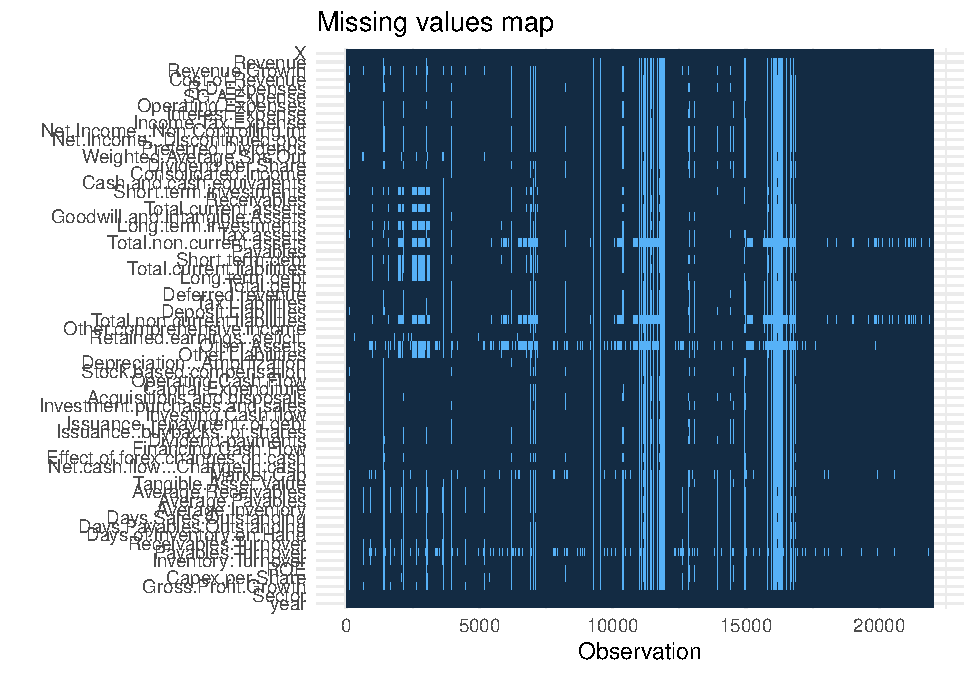
\includegraphics{stock_analysis_files/figure-latex/missing values-1} 

}

\caption{Missing values map before imputation}\label{fig:missing values}
\end{figure}

To account for missing values, we chose to use the CART (Classification
and Regression Trees) method of imputation. After imputation, 4 columns
still had missing values, which were then subsequently removed.

\hypertarget{correlation-plot}{%
\subsection{Correlation Plot}\label{correlation-plot}}

There were 61 columns after we finished data cleaning and we wanted to
select only significant features for our target variable before
modeling. Before focusing on feature selection, we had to check for
correlation between the independent variables. We performed a
correlation analysis based on Pearson's coefficient between each numeric
predictor first. We considered a \textbar correlation\textbar{}
\textgreater{} 0.8, with p \textless{} 0.05 as a significant
correlation. Figure 2 demonstrates significant correlation between many
of our predictor variables. However, due to the large amount of
variables, the correlation plot was not interpretable if all the
variables were plotted together. Therefore, we filtered the correlation
plot by keeping only variables that had a correlation with absolute
value greater than 0.8.

\begin{figure}

{\centering 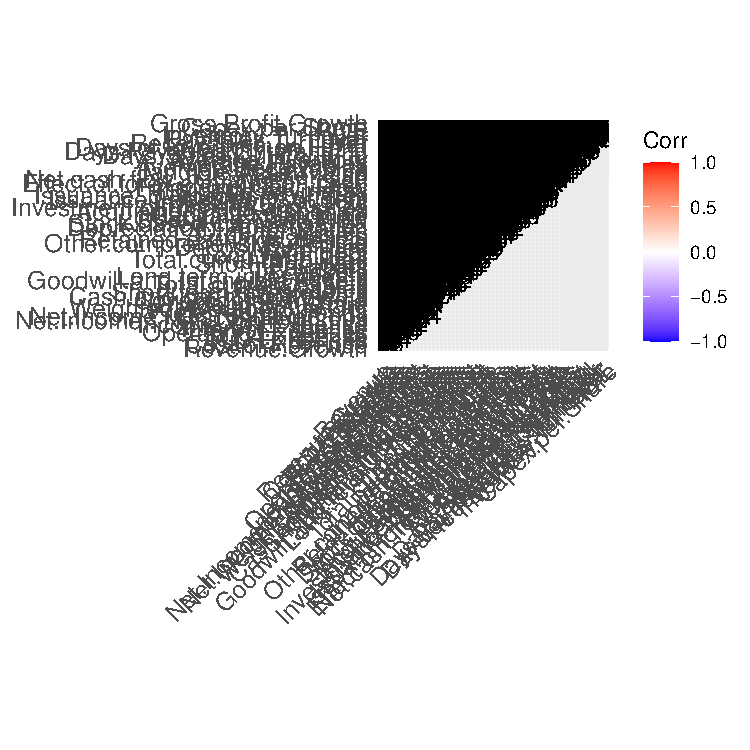
\includegraphics{stock_analysis_files/figure-latex/corrplot-1} 

}

\caption{Correlogram of variables with |R| > 0.8}\label{fig:corrplot}
\end{figure}

\hypertarget{data-distribution}{%
\subsection{Data Distribution}\label{data-distribution}}

We to observe the means, and check for outliers. Most variables were not
normally distributed and had a clear skew. In Figure 3, we show a subset
of the variable distributions.

\begin{figure}

{\centering 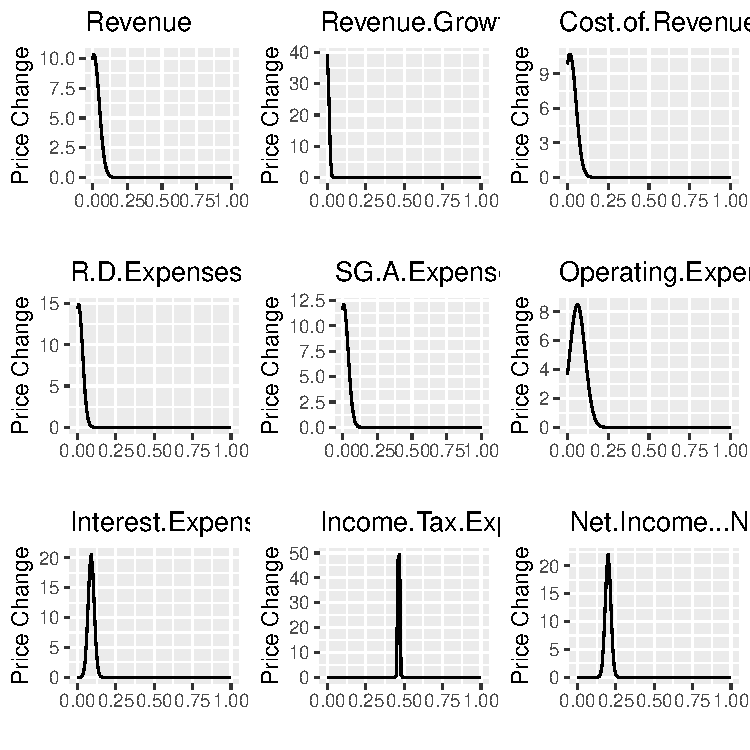
\includegraphics{stock_analysis_files/figure-latex/data normal distribution plot1-1} 

}

\caption{Column distributions}\label{fig:data normal distribution plot1}
\end{figure}

\hypertarget{feature-selection-1}{%
\subsection{Feature Selection}\label{feature-selection-1}}

Since there were 61 columns on our dataset, we ran a decision tree model
to determine the most important variables to be included in predicting
market cap. Below are plots showing the importance of each variable. We
also ran a correlation to ensure that the features were not highly
correlated. The top 10 important variables were: consolidated income,
dividend payments, stock based compensation, income tax expense,
retained earnings deficit, operating cash flow, operating expenses, R \&
D expenses, total debt, and long term debt.

\begin{figure}

{\centering 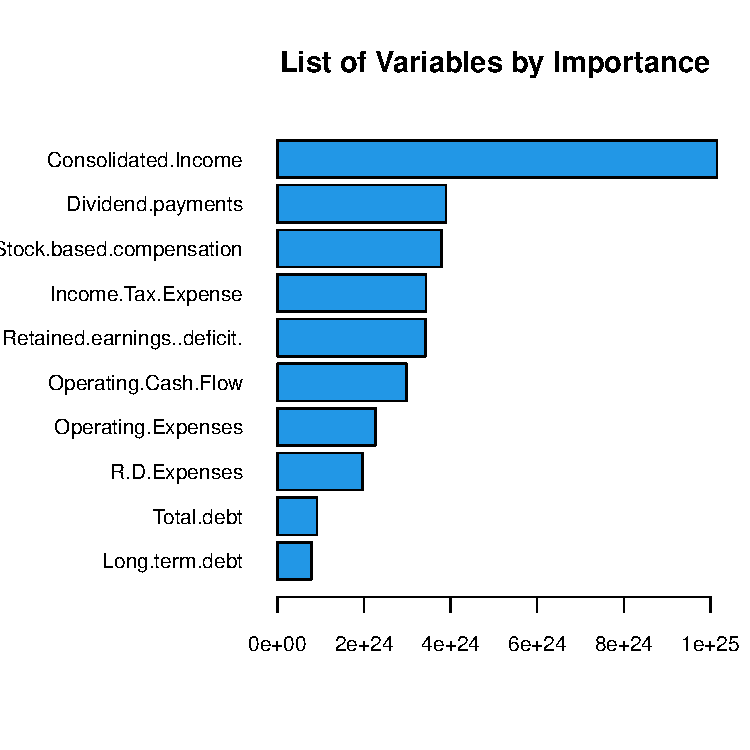
\includegraphics{stock_analysis_files/figure-latex/variable importance-1} 

}

\caption{Top 10 variable importance, determined by Decision Tree}\label{fig:variable importance}
\end{figure}

\begin{figure}

{\centering 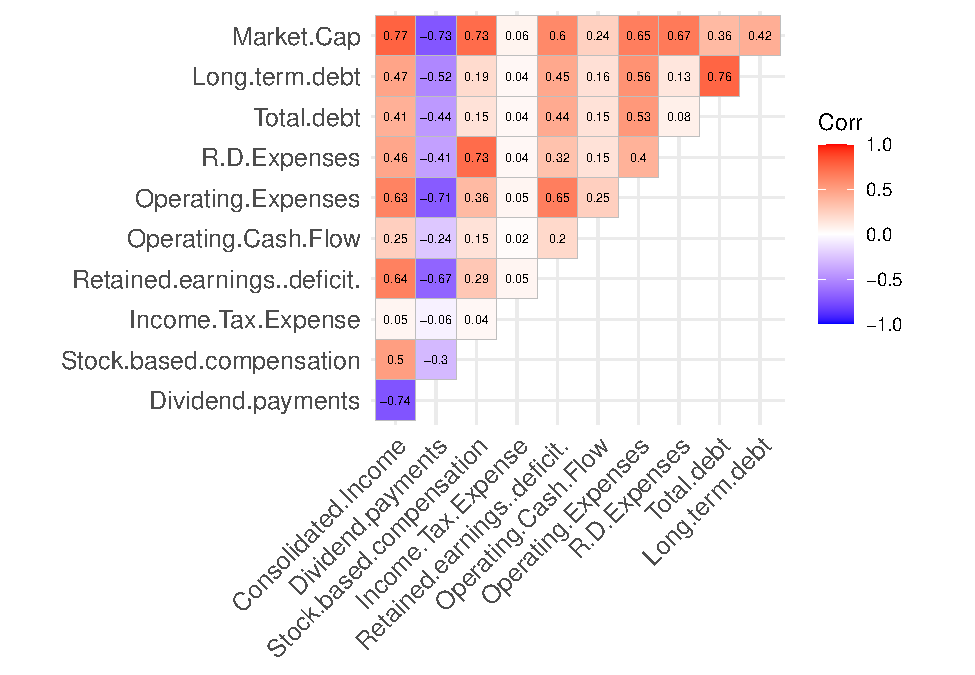
\includegraphics{stock_analysis_files/figure-latex/correlation plot 2-1} 

}

\caption{Correlogram of Top 10 Variables}\label{fig:correlation plot 2}
\end{figure}

\hypertarget{principal-component-analysis-1}{%
\subsection{Principal Component
Analysis}\label{principal-component-analysis-1}}

We performed PCA to reduce the dimensionality of our feature dataset.
The Scree plot (Figure 6) shows the overall variance explained by each
principal component. The top 5 dimensions explained approximately 90\%
of the total variance within the data. Individual datapoints involving
large technology companies (Google, Apple, Amazon) had high
contributions to the overall variance (Figure 7). R\&D Expenses and
Stock-based compensation were two variables with high contribution to
variance, while Income Tax Expense and Operating Cash Flow had more
negligible contribution (Figure 8).

\begin{figure}

{\centering 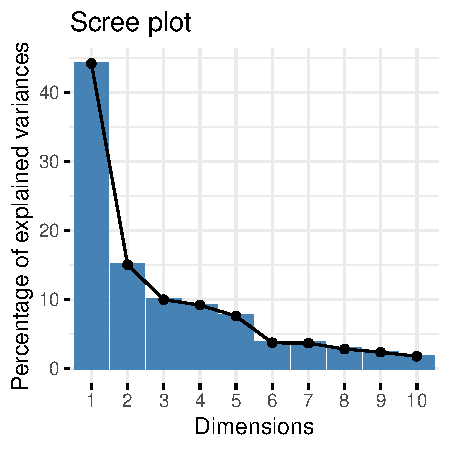
\includegraphics{stock_analysis_files/figure-latex/scree-1} 

}

\caption{Scree plot}\label{fig:scree}
\end{figure}
\begin{figure}

{\centering 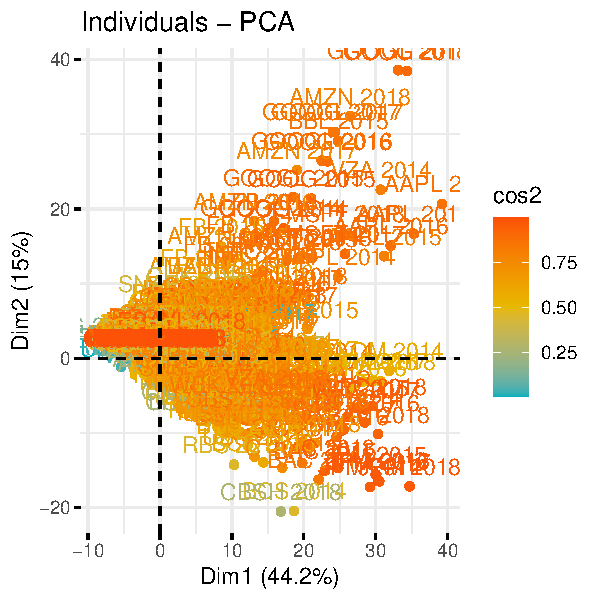
\includegraphics{stock_analysis_files/figure-latex/PCAind-1} 

}

\caption{Effect of Individual points - PCA}\label{fig:PCAind}
\end{figure}
\begin{figure}

{\centering 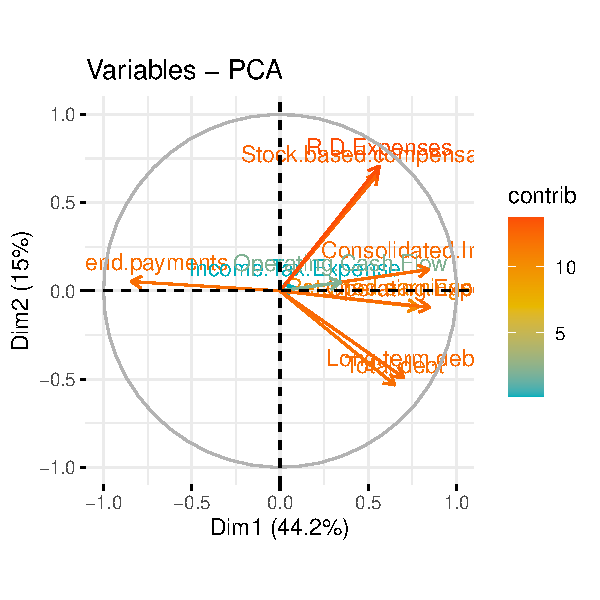
\includegraphics{stock_analysis_files/figure-latex/PCAvar-1} 

}

\caption{Effect of Variables - PCA}\label{fig:PCAvar}
\end{figure}

\hypertarget{k-means-clustering}{%
\subsection{K Means Clustering}\label{k-means-clustering}}

The ``silhouette'' method was first performed to determined number of
clusters. It suggested a number of cluster of 2 (k=2). The `elbow
method' was then performed to determine an optimal number of k clusters.
However, there was no significant drop in within-cluster sum of squares
with k besides k=2. As two clusters did not provide much discrimination
for our observations, we instead used k=4 as the final number of
clusters.

\begin{figure}

{\centering 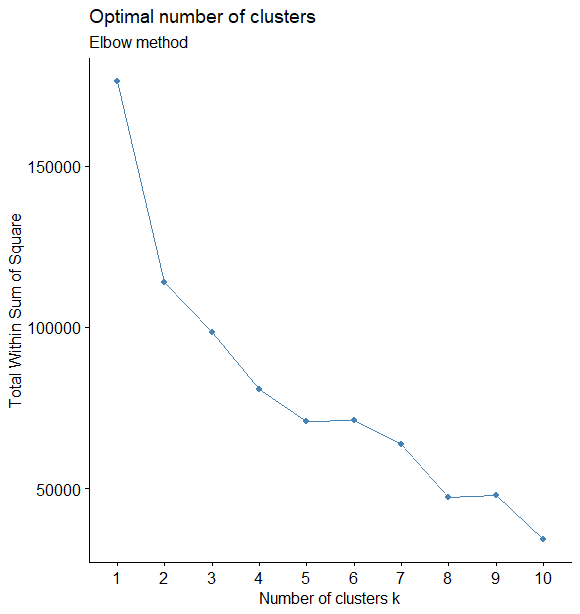
\includegraphics[width=0.6\linewidth,height=0.4\textheight]{unsupervised_elbow} 

}

\caption{Elbow method}\label{fig:elbow}
\end{figure}

The following figure displays our datapoints in a 2-D space based on 4
clusters.

\begin{landscape}
\begin{figure}
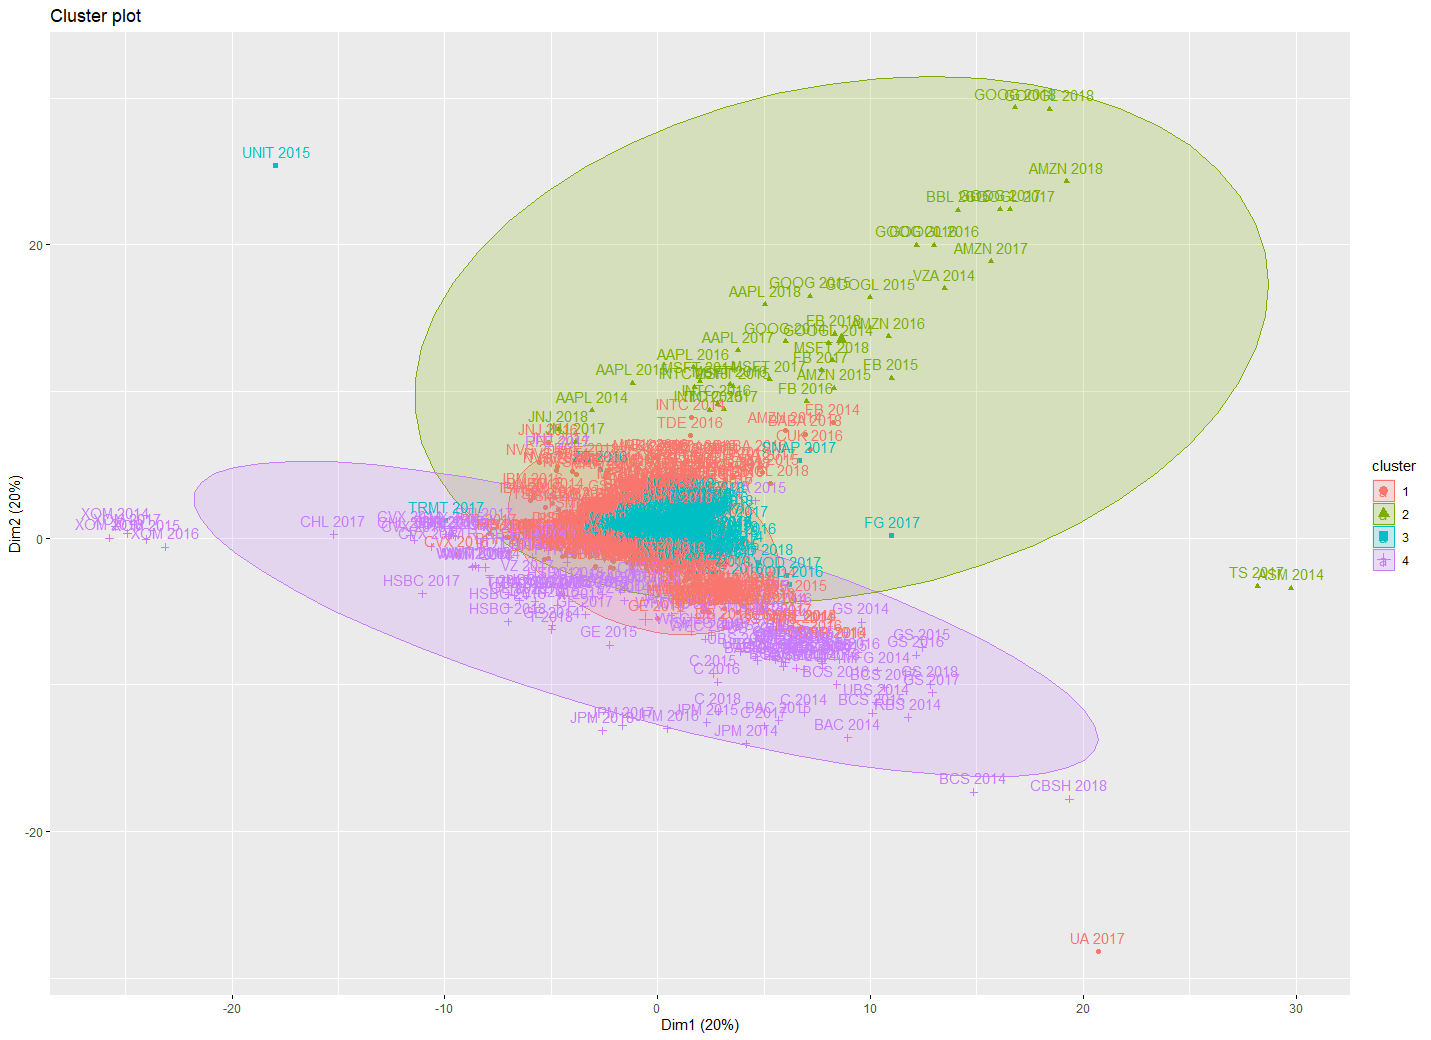
\includegraphics[width=1\linewidth,height=1\textheight]{cluster_image} \caption{K means clustering, k = 4}\label{fig:cluster}
\end{figure}
\end{landscape}

\hypertarget{cluster-interpretation}{%
\subsection{Cluster Interpretation}\label{cluster-interpretation}}

We performed some exploratory visualizations to interpret how the data
was clustered by k-means. Cluster 1 contained the majority of
observations, with n=19759. Cluster 2 had 35 observations, cluster 3 had
126, and cluster 4 had 586. On average, cluster 1 contained more small-
and medium-sized companies compared to other clusters, with 89\% of
observations falling under a market cap of \$10 billion.\\

\begin{figure}

{\centering 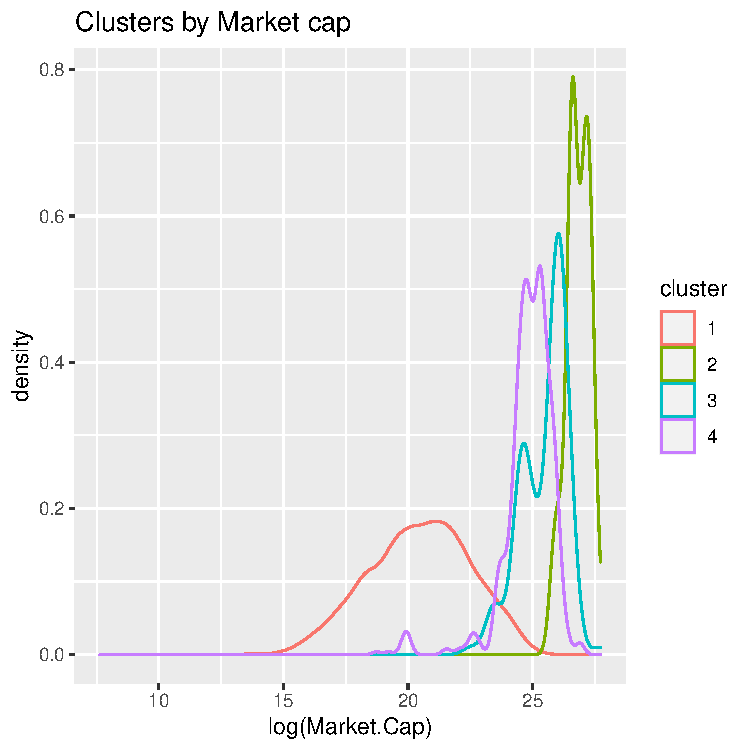
\includegraphics{stock_analysis_files/figure-latex/cluster by marketcap-1} 

}

\caption{Clusters by Market Cap}\label{fig:cluster by marketcap}
\end{figure}

K-means was able to segregate the large high-tech companies: Facebook,
Apple, Amazon, Google, Intel, and Microsoft all into one cluster
(Cluster 2). We noted that these companies trended towards large market
capitalization, high stock compensation, and high R \& D expenses.
Cluster 3 contained a significant majority of big banks, such as JP
Morgan, Wells Fargo, and Bank of America, as well as large energy
corporations such as ExxonMobil and Chevron. Clusters 1 and 4 had
similar sector distributions, although companies in cluster 4 were all
large cap. Interesting to note that the top 20 big pharmaceutical and
healthcare companies were mainly in cluster 4, such as Johnson \&
Johnson, Roche, and Abbvie.\\

\begin{figure}

{\centering 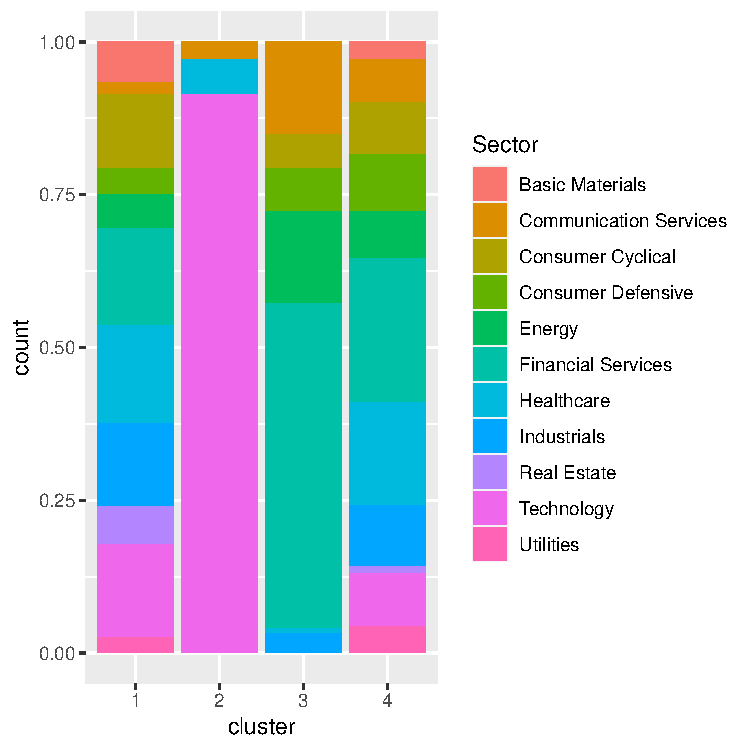
\includegraphics{stock_analysis_files/figure-latex/sector-1} 

}

\caption{Clusters by Sector}\label{fig:sector}
\end{figure}

Price-to-earnings ratio is a common method of determining how a company
is valued by investors. A high P/E ratio may suggest that investors are
willing to pay a higher price for that company's share price because of
future growth expectations. Here, we see that cluster 2, composed
largely of high-tech companies such as Google, had high P/E ratios -
aligning with investor sentiments about the growth of the industry.
Cluster 1 maintains an interesting bimodal distribution of positive and
negative P/E ratios. Stocks with negative P/E ratio suggest that these
companies are reporting a loss.

\begin{figure}

{\centering 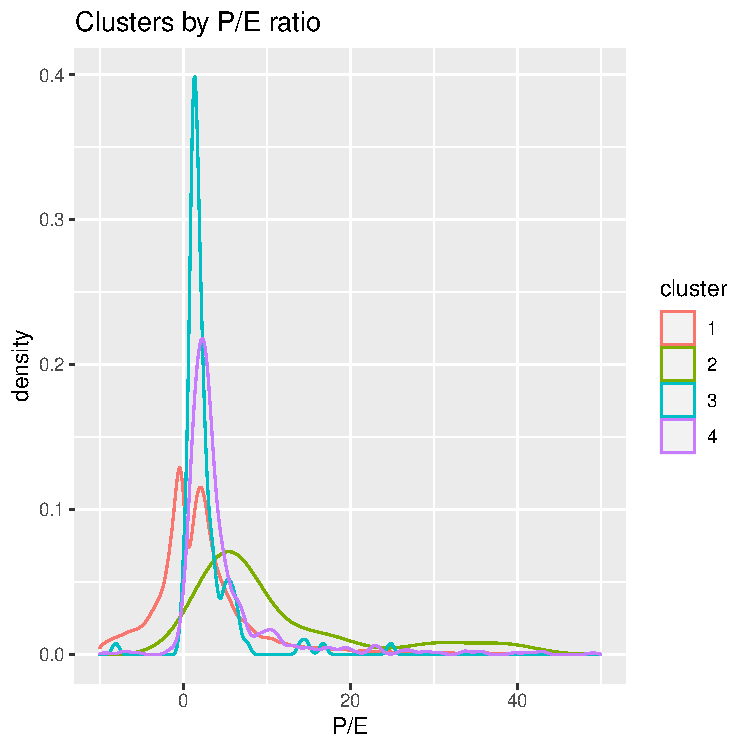
\includegraphics{stock_analysis_files/figure-latex/pe ratio-1} 

}

\caption{Clusters by P/E ratio}\label{fig:pe ratio}
\end{figure}

Normalizing for the proportion of small-medium and large cap stocks in
cluster 1, we noted that small to medium-sized companies were 2 to 3
times more likely to have a negative P/E ratio compared to large
companies. The bimodal distribution in cluster 1 can therefore be
partially explained by a split between the distribution of company size.

\begin{figure}

{\centering 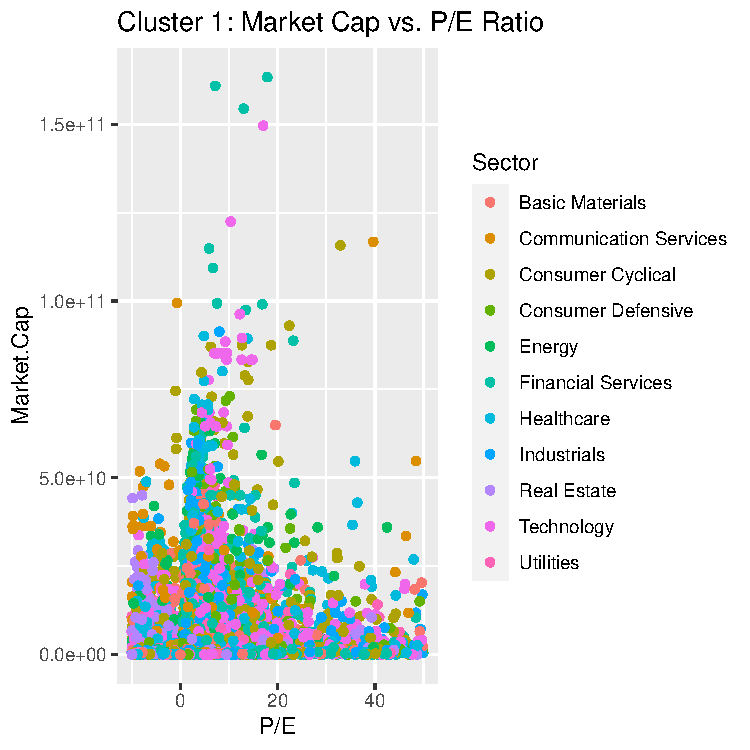
\includegraphics{stock_analysis_files/figure-latex/pe ratio clust1-1} 

}

\caption{Cluster 1: Market Cap vs. P/E Ratio}\label{fig:pe ratio clust1}
\end{figure}

\hypertarget{modeling}{%
\subsection{Modeling}\label{modeling}}

K-fold cross-validation method was used to train the models instead of
the simple train-test-split for this project, as it gives a more valid
estimation of model effectiveness. The k-fold cross-validation method
evaluates the model performance on different subsets of the training
data and calculates the average prediction error rate. For this value
k=10 was used on all models.

\hypertarget{xgboost}{%
\subsection{XGBoost}\label{xgboost}}

The XGBoost model was used and was parametrized using grid method. The
final parameter values used by the best model were nrounds = 200,
max\_depth = 6, eta = 0.1, gamma = 0, colsample\_bytree = 0.5,
min\_child\_weight = 1 and subsample = 0.8.

\begin{figure}

{\centering 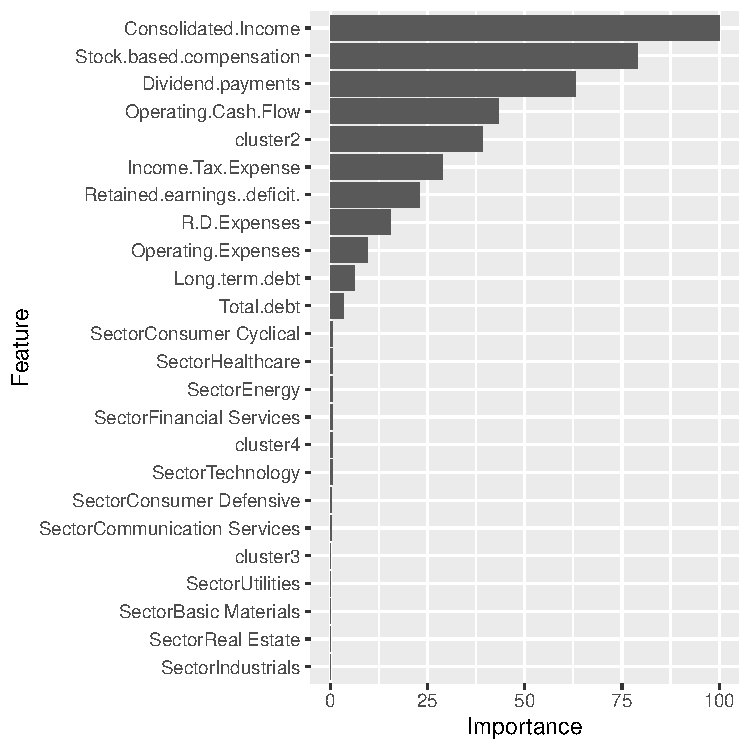
\includegraphics{stock_analysis_files/figure-latex/XGBoost-1} 

}

\caption{XGBoost Tuning Parameters}\label{fig:XGBoost-1}
\end{figure}
\begin{figure}

{\centering 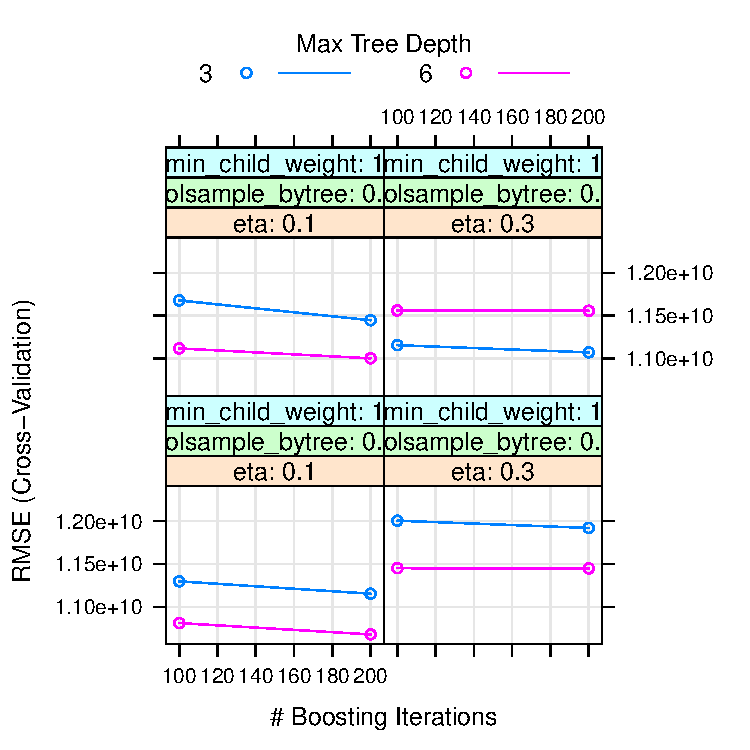
\includegraphics{stock_analysis_files/figure-latex/XGBoost-2} 

}

\caption{XGBoost Tuning Parameters}\label{fig:XGBoost-2}
\end{figure}
\begin{figure}

{\centering 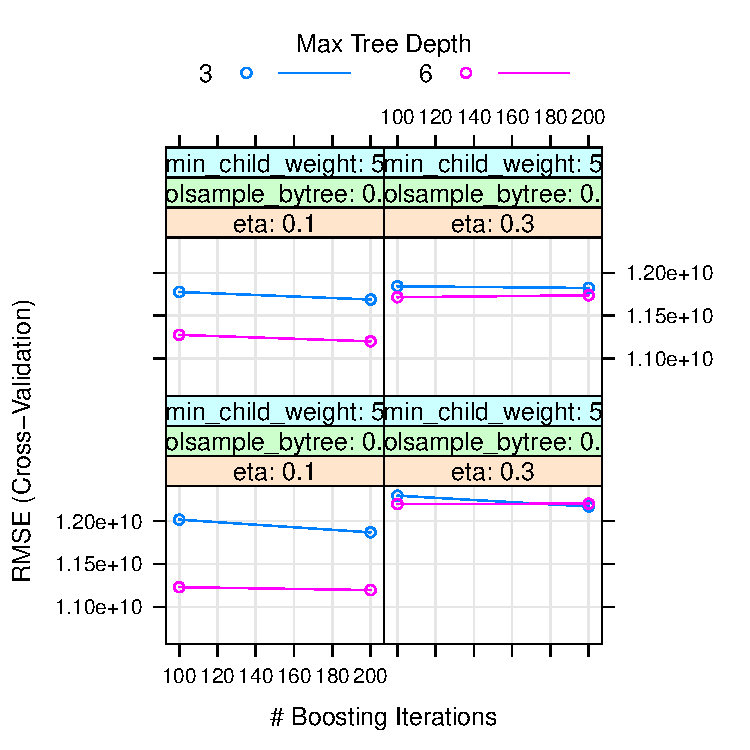
\includegraphics{stock_analysis_files/figure-latex/XGBoost-3} 

}

\caption{XGBoost Tuning Parameters}\label{fig:XGBoost-3}
\end{figure}

\hypertarget{gradient-boosting}{%
\subsection{Gradient Boosting}\label{gradient-boosting}}

The gradient boosting model was tuned by several parameters. The final
values used for the model were n.trees = 600, interaction.depth = 9,
shrinkage = 0.1 and n.minobsinnode = 20

\begin{center}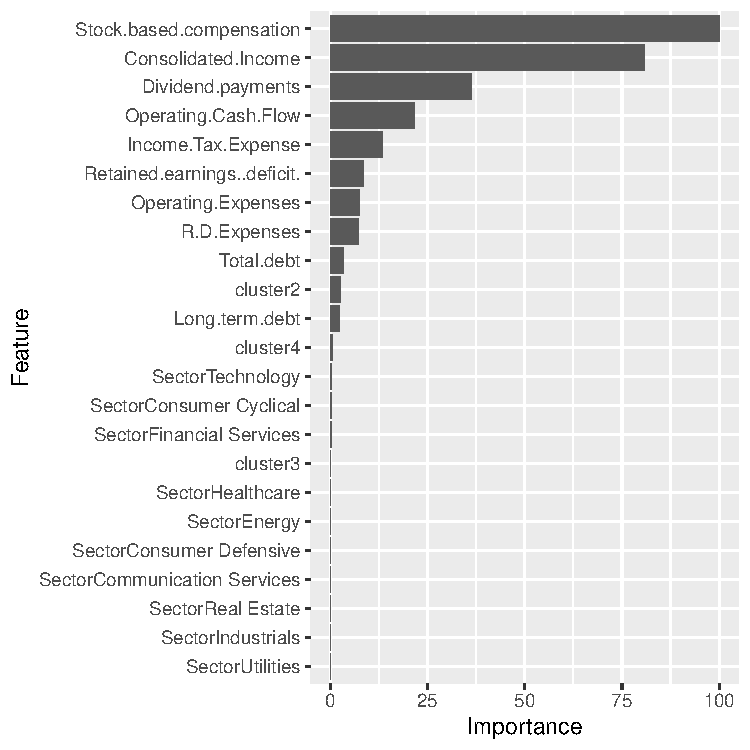
\includegraphics{stock_analysis_files/figure-latex/gradient boosting-1} \end{center}

\hypertarget{random-forest}{%
\subsection{Random Forest}\label{random-forest}}

The Random Forest model was ran using its normal parameters. The model
automatically tunes with one parameter mtry. The final model used mtry =
12.

\hypertarget{model-selection}{%
\subsection{Model Selection}\label{model-selection}}

All models found \(Consolidated Income\), \(Stock based Compensation\)
and \(Dividend Payments\) to be important predictors of Market.Cap. Mean
Absolute Error (MAE) shows the average error of the predicted variable.
Root Mean-Squared Error (RMSE) is similar with MAE but it is more useful
when we are interested in fewer large errors over many small errors.
Overall, we prioritized model stability by prioritizing RMSE over MAE.
\(R^2\) computes how well the regression model fits the data. The higher
the \(R^2\) value, the better the model fits the data. For predicting
market cap, we desired a model with the lowest RMSE and MAE to keep the
high accuracy of prediction. The XGBoost model had the highest \(R^2\)
as well as the lowest RMSE and MAE, thus, it was chosen for deployment.

\begin{longtable}[]{@{}llrl@{}}
\caption{Model Accuracy}\tabularnewline
\toprule
model & RMSE & R2 & MAE\tabularnewline
\midrule
\endfirsthead
\toprule
model & RMSE & R2 & MAE\tabularnewline
\midrule
\endhead
random\_forest & 1.10e+10 & 0.89 & 2.56e+09\tabularnewline
extreme\_gradient\_boosting & 1.08e+10 & 0.90 & 2.70e+09\tabularnewline
gradient\_boosting & 1.18e+10 & 0.88 & 2.92e+09\tabularnewline
\bottomrule
\end{longtable}

\hypertarget{discussion}{%
\section{Discussion}\label{discussion}}

This project focused on applying unsupervised and supervised learning on
stock data. We merged 5 datasets from different years of stock data with
the same attributes, containing a total of 225 columns. We cleaned the
data by choosing fundamental columns and imputing missing values using
the MICE package. We then ran a decision tree model which chose the most
important variables which were used as the features for our modeling.

Unsupervised learning using the K-means algorithm was used to cluster
the data into 4 different clusters. Cluster 1 was the largest and had
19759 observations. It included small-medium sized companies, where 89\%
of the observations fell under a market cap of \$10 billion. Cluster 2
was the smallest with 35 observations and it included the large
high-tech companies, such as Amazon, Apple, Facebook and Google. Cluster
3 had 126 observations and included majority of the big banks such as
Bank of America and large energy corporations such as Chevron. Cluster 4
had 568 observations similar sector distribution to cluster one,
however, the companies all had a large market cap. In this cluster 20
large pharmaceutical and healthcare companies were found. It was
interesting to see how well the clustering algorithm was able to cluster
the data in different sections based on the type of company they were,
their market cap and other attributes. However, it is notable to discuss
that the clusters were not equally distributed and cluster 1 was harder
to interpret due to the large number of observations. A larger number of
cluster could be considered in future work in order to make the clusters
smaller and more interpretable. It is important to note that both the
elbow method and silhouette method to chose the number of clusters
suggested a cluster number of 2, which when was ran resulted in a very
large cluster and a negligible second cluster. Thus, we observed that
algorithms determining cluster numbers should be used as a guide and
tuned when needed. We also learned that it is important to change the
number of cluster to make the data as interpretable as possible.

Supervised learning was applied on the 10 important features plus Sector
and cluster \# as features. Three algorithms, XGBoost, GBM and Random
Forest were ran using the cross-validation method. XGBoost and GBM
models were tuned with several parameters, while Random Forest was not
due to its high running time. The models were evaluated using \(R^2\),
RMSE and MAE and XGBoost was the best performer, with Random Forest
being the second best and GBM being the worst performer. It is important
to note that Random Forest performed almost as well as XGBoost without
tuning, thus, if the model was tuned it could have achieved higher
performance then the XGBoost. However, this was not possible due to the
short time frame of this project and the running time of the model.
Therefore, we realized that it is important to consider modeling running
time and project timeline when choosing our models. XGBoost achieved a
\(R^2\) value of 0.9010295. This means that the std (standard deviation)
of the error of the regression model is 1/3 of the std of the error that
would be achieved with a constant-only model (a regression model without
predictors). Thus the model is quite accurate in prediction, however,
there is still error present. A higher \(R^2\) value and lower RMSE and
MAE values could have been achieved if the model parameters were tuned
further. However, due to the limited time frame, the model's parameters
were tuned only by values, rather then value range. Using value range
instead of values on the grid tuning algorithm would have allowed for
more possibility of achieving a more highly accurate model.

Our project had several limitations. First of all the data was old, from
2014-2018 and may not reflect the situation of the stocks currently. In
addition, it is important to note that COVID-19 has dramatically changed
the economy and affected the prices of stocks - for example, inflating
even further the price of tech stocks. Thus, while using this app, users
might not get a reflection of the current marketplace. Furthermore, the
supervised learning gave many unbalanced clusters, one of them
containing 19759 observations, which was hard to interpret. Thus, this
could have given error in our interpretation of the cluster. In
addition, these clusters were used in our modelling, thus the unbalanced
or non-interpretable clusters could misguide the users. Additionally, we
assumed that the market capitalization of the data fairly represented
the intrinsic value of the company. Price discovery may have occurred
between the time that these data were collected and the current economy.

\hypertarget{ethical-considerations}{%
\subsection{Ethical considerations}\label{ethical-considerations}}

It is important to note that this app uses historic data, thus it is not
to be used as a perfect prediction of the current marketplace.
Predictions offered by this application are not to be used completely
place of advice from finance professionals or due diligence. Research
has shown that on average, most investors cannot beat the market; the
stock market is a zero-sum game. While these predictions might aid in
picking individual stocks, investing in a broadly-diversified
exchange-traded fund (ETF) is one method to ensure consistent, long-term
gains.

\newpage

\hypertarget{bibliography}{%
\section{Bibliography}\label{bibliography}}

Advanced Technical Analysis Concepts {[}Internet{]}. Investopedia.
{[}cited 2020 Nov 11{]}.~ Available from:
\url{https://www.investopedia.com/advanced-technical-analysis-concepts-4689656}\\
Boyte-White C. Revenue vs.~Income: What's the Difference?
{[}Internet{]}. Investopedia.~ {[}cited 2020 Nov 11{]}. Available
from:~\url{https://www.investopedia.com/ask/answers/122214/what-difference-between-revenue-and-income.asp}
Chen T, Guestrin C. Xgboost: A scalable tree boosting system.
InProceedings of the 22nd acm sigkdd international conference on
knowledge discovery and data mining 2016 Aug 13 (pp.~785-794).\\
Hayes A. Price-to-Earnings Ratio -- P/E Ratio {[}Internet{]}.
Investopedia. {[}cited 2020 Nov 11{]}. Available
from:~\url{https://www.investopedia.com/terms/p/price-earningsratio.asp/}
Majaski C. The Difference Between Fundamental vs.~Technical Analysis?
{[}Internet{]}.~ Investopedia. {[}cited 2020 Nov 11{]}. Available
from:\\
Natekin A, Knoll A. Gradient boosting machines, a tutorial. Frontiers in
neurorobotics. 2013 Dec
4;7:21.https://www.investopedia.com/ask/answers/difference-between-fundamental-and-technical-analysis/
Staff I. Can Stocks have a negative price-to-earnings ratio?
{[}Internet{]}. Investopedia. {[}cited 2020 Nov 11{]}. Available
from:~\url{https://www.investopedia.com/ask/answers/05/negativeeps.asp}\\
Strader TJ, Rozycki JJ, Root TH. Machine Learning Stock Market
Prediction Studies: Review and Research Directions. 2017;28(4):22. Teng
X, Wang T, Zhang X, Lan L, Luo Z. Enhancing Stock Price Trend Prediction
via a Time-Sensitive Data Augmentation Method {[}Internet{]}. Vol. 2020,
Complexity. Hindawi; 2020 {[}cited 2020 Nov 10{]}. p.~e6737951.
Available
from:~\url{https://www.hindawi.com/journals/complexity/2020/6737951/}
The Complete List of Bank Stocks Trading on the NYSE \textbar{}
TopForeignStocks.com {[}Internet{]}. {[}cited 2020 Nov 11{]}. Available
from:~\url{https://topforeignstocks.com/stock-lists/the-complete-list-of-bank-stocks-trading-on-the-nyse-2/}
Zhong X, Enke D. Predicting the daily return direction of the stock
market using hybrid machine learning algorithms. Financ Innov. 2019
Dec;5(1):1--20.





\newpage
\singlespacing 
\end{document}
